\section{Optimisation et amélioration du nouveau modèle}
%opti 1
	%addcat
	%reprise train
	%batch
%pb mémoire (beaucoup d'opti perf nécessite d'augmenter la taille des params/modules/tenseurs...) & tps (la plupart des otpis perfs augmentent le tps de calcul nécessaire, et de base le modele naif est trop lent)
%pb memoire réglé, tentative infructueuse d'améliorer les perfs avec améliorations préparées en parallèle
	%+ params
	%lbl
% ccl plus pb mémoire & tps, opti z'oignons (XD) même, 5 min c'est balèze

Une fois le prototype fonctionnel, nous avons amélioré ses performances.
Par performances, nous entendons principalement le temps nécessaire pour que la qualité prédictive du modèle dépasse un certain seuil.

Pour améliorer ce temps d'entraînement, il est possible de travailler sur deux dimensions~:
\begin{itemize}
	\item la \emph{quantité de \glspl{data}} traitées en un laps de temps~;
	pour cela on peut optimiser les algorithmes et le modèle pour réduire le temps nécessaire pour traiter les \glspl{example}~;
	c'est une \emph{stratégie quantitative}~;
	\item la \emph{qualité} de l'apprentissage pour une quantité fixée de \glspl{data}~;
	pour cela on peut améliorer le modèle en réglant les paramètres (comme la fréquence de transmission) ou en implémentant de nouvelles mécaniques~;
	c'est une \emph{stratégie qualitative}.
\end{itemize}

Les deux stratégies ont été utilisées. Il faut noter que certaines améliorations qualitatives ont un impact quantitatif négatif.

Principalement, le travail effectué pendant cette partie du projet est un travail de débogage, d'analyse et d'optimisation, avec peu d'implémentation de nouvelles mécaniques dans le \gls{model}.

\subsection[Agrégation des sorties des couches]{Agrégation des sorties des couches~: d'une stratégie additive à une concaténation}\label{subsec:addcat_}
La première optimisation a été de changer la façon de regrouper les informations de toutes les \og échelles\fg{} avant de les transmettre au module produisant la distribution de probabilité.

Initialement, les sorties de toutes les \og échelles\fg{} étaient sommées. Cela permettait de maintenir des \glspl{tensor} de dimensions uniformes quel que soit le nombre d'\og échelle\fg{} (voir figure \ref{fig:add}, \autopageref{fig:add}).

Après discussion avec le maître de stage, la stratégie d'agrégation à été changé en une concaténation des sorties.

Comme montré dans la figure \ref{fig:cat} (\autopageref{fig:cat}), les sorties sont mises côte-à-côte afin de former un nouveau \gls{tensor} et la taille du \gls{tensor} concaténé change en fonction du nombre d'entrées.
La manipulation de \glspl{tensor} de taille non fixée est très ardue dans ce cas précis, bien que nous ne développerons pas plus avant les raisons de cette difficulté.

Cela a nécessité l'abandon de la propriété de croissance à l'infini de l'architecture (décrite \autoref{inf_growth}, \autopageref{inf_growth}), au profit d'un nombre maximal d'échelles défini à l'avance ou déterminée à l'aide d'une formule en fonction des données disponibles (décrite \mbox{\autoref{growth_formula}}, \autopageref{growth_formula}).

\begin{figure}[ht]
	\begin{subfigure}{0.45\textwidth}
		\centering
		\scalebox{1}{\def\layersep{5em}
\begin{tikzpicture}[shorten >=1pt,->,draw=black, node distance=\layersep]
\tikzstyle{every pin edge}=[<-,shorten <=1pt]
\tikzstyle{block}=[minimum size=2em];
\tikzstyle{value}=[rectangle, fill=green!50,block];
\tikzstyle{operation}=[block, circle,inner sep=0pt, fill=red!50];
\tikzstyle{nonlinearity}=[rectangle,block, fill=blue!50];
\tikzstyle{annot} = [text width=6em, text centered]

% Draw the input layer nodes
\foreach \name / \y in {1,...,3}
% This is the same as writing \foreach \name / \y in {1/1,2/2,3/3,4/4}
\node[value, label={[]north:{\'{E}chelle \y}}] (I-\name) at (0,-2*\y) {\y};
\node[value, label={[]north:{\'{E}chelle 4}}, opacity=.5] (I-4) at (0,-8) {4};

% Draw the output layer node
\node[operation, right of=I-2] (ope) {{\Large +}};
\node[value, right of=ope, label={[]north:$1+2+3+4$}](cat){};
% Draw the output layer node
%\node[nonlinearity, right of=cat] (lin) {Lin};
%\node[annot, right of=lin, text width=7em,xshift=2em ] (out) {Distribution de probabilit\'{e}s};

% Connect every node in the input layer with every node in the
% hidden layer.
\foreach \source in {1,...,3}
\path (I-\source.east) edge (ope);
\path (I-4.east) edge[dashed, opacity=.5] (ope);
\path (ope) edge (cat);
%\path (cat) edge (lin);
%\path (lin) edge (out);
\end{tikzpicture}}
		\caption[Stratégie d'agrégation additive]{Stratégie d'agrégation additive}\label{fig:add}
	\end{subfigure}
	\begin{subfigure}{0.45\textwidth}
		\centering
		\scalebox{1}{\def\layersep{5em}
\begin{tikzpicture}[shorten >=1pt,->,draw=black, node distance=\layersep]
    \tikzstyle{every pin edge}=[<-,shorten <=1pt]
    \tikzstyle{block}=[minimum size=2em];
    \tikzstyle{value}=[rectangle, fill=green!50,block];
    \tikzstyle{operation}=[block, circle,inner sep=0pt, fill=red!50];
    \tikzstyle{nonlinearity}=[rectangle,block, fill=blue!50];
    \tikzstyle{annot} = [text width=6em, text centered]

    % Draw the input layer nodes
    \foreach \name / \y in {1,...,3}
    % This is the same as writing \foreach \name / \y in {1/1,2/2,3/3,4/4}
        \node[value, label={[]north:{\'{E}chelle \y}}] (I-\name) at (0,-2*\y) {\y};
	\node[value, label={[]north:{\'{E}chelle 4}}, opacity=.5] (I-4) at (0,-8) {4};

    % Draw the output layer node
    \node[operation, right of=I-2] (ope) {Cat};
    \node[value, right of=ope](cat){2};
    \node[value, above of=cat, node distance=2.1em]{1};
    \node[value, below of=cat, node distance=2.1em](3){3};
    \node[value, below of=3, node distance=2.1em, opacity=.5]{4};
    % Draw the output layer node
    \node[nonlinearity, right of=cat] (lin) {Lin};
	\node[annot, right of=lin, text width=7em,xshift=2em ] (out) {Distribution de probabilit\'{e}s};

    % Connect every node in the input layer with every node in the
    % hidden layer.
    \foreach \source in {1,...,3}
        \path (I-\source.east) edge (ope);
	\path (I-4.east) edge[dashed, opacity=.5] (ope);
	\path (ope) edge (cat);
	\path (cat) edge (lin);
	\path (lin) edge (out);
\end{tikzpicture}}
		\caption[Stratégie d'agrégation par concaténation]{Stratégie d'agrégation par concaténation}\label{fig:cat}
	\end{subfigure} 
	\caption{Stratégies d'agrégation}
\end{figure}

La stratégie par concaténation est plus lente en terme de temps de calcul que la stratégie additive, cependant pour le même temps de calcul elle permet d'obtenir de meilleurs résultats. La figure \ref{fig:addcat} (\autopageref{fig:addcat}) représente ces résultats. Le temps de calcul alloué à l'entraînement des deux modèles est identique. Avec la concaténation on entraîne le modèle sur 1/4 des données, avec l'addition on l'entraîne 5 fois sur l'ensemble des données. Avec la concaténation, on obtient un BPC de 3.5, alors qu'on obtient un BPC de 4 avec l'addition.

Plus de détail sur le choix de la stratégie d'agrégation sont disponibles dans l'annexe \ref{subsec:addcat} (\autopageref{subsec:addcat}). 

\begin{figure}[H]
	\centering
	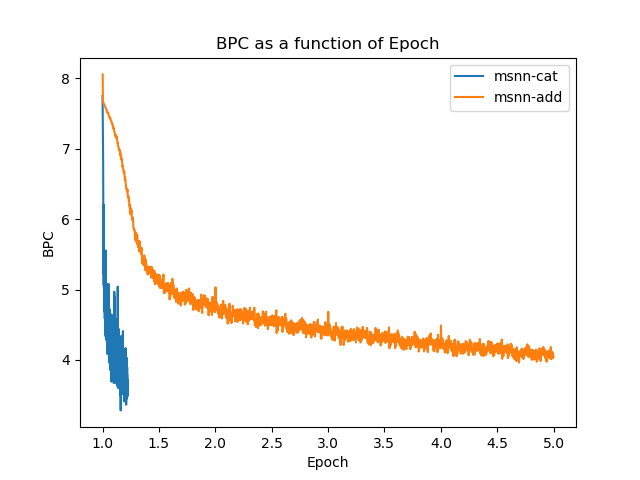
\includegraphics[width=\textwidth]{parts/appendix/reports-gmsnn/docs_esteban-latex/test_reports/comparative-bpc-msnn-det-msnn-cat.png}
	\caption[Performances comparées des stratégies additive et par concaténation]{Performances comparées des stratégies par concaténation \textit{(msnn-cat)} et additive \textit{(msnn-add)}}\label{fig:addcat}
\end{figure} % new
\subsection{Sauvegarde, interruption et reprise de l'entraînement}\label{subsec:gmsnn_save}
Une fonctionnalité s'est très vite détachée comme essentielle~: la sauvegarde du \gls{model}, et l'interruption et la reprise de l'entraînement.

En effet, avec des entraînements très lents et donc longs, il était nécessaire de pouvoir suspendre l'entraînement afin de répartir le temps d'entraînement sur plusieurs sessions de plusieurs heures. De plus, les sauvegardes permettaient de conserver le modèle une fois qu'il est entraîné.

Le système implémenté permet d'effectuer cycliquement des sauvegarde du modèle ainsi que de l'état de l'entraînement, permettant ainsi une reprise en l'état de l'entraînement.

Pour la réalisation du système, le principal obstacle à été le malfonctionnement initial des outils fournis par \gls{pytorch}.
Cela à poussé à la conception d'un système de sauvegarde personnalisé mais malheureusement assez complexe.
Cependant, la mise-à-jour majeure de la librairie qui c'est déroulé à point nommé à résolu le problème, et c'est avec les outils de \gls{pytorch} que le système de sauvegarde à finalement été implémenté.

Voir l'annexe \ref{subsec:save} pour un rapport contenant plus de détail sur le système de sauvegarde. % new
\subsection{Tentatives d'optimisation, fuites de mémoire et lenteur de l'entraînement}\label{subsec:optimem}

Les optimisations testées par la suite ont révélé des fuites de mémoire et mis en lumière une lenteur excessive de l'apprentissage.

Les optimisations en question ont été suspendues le temps de la résolution de ces deux problèmes.
Il s'agit de~:
\begin{itemize}
	\item l'utilisation de \glspl{batch} simultanés (voir \autoref{subsec:optibatch}, \autopageref{subsec:optibatch})~; 
	\item l'augmentation du nombre de \glspl{parameter} du \gls{model} (voir \autoref{subsec:optiparam}, \autopageref{subsec:optiparam})~;
\end{itemize}

%\hspace{1em}
\subsubsection{Consommation de mémoire et de temps de calcul accrue}
Un effet direct des optimisations testées est l'augmentation de la consommation de mémoire.

Cette consommation accrue a causé le plantage\footnote{Un plantage en informatique est l'arrêt d'un programme causé par un dysfonctionnement.} de plusieurs tests, révélant la présence de fuites critiques de mémoire.
Un ralentissement progressif de l'entraînement a aussi été mis en évidence pendant l'analyse du problème.
Le plus surprenant a été la corrélation forte observée entre le temps de calcul et la consommation de mémoire.

Un premier correctif a fourni une amélioration notable mais insuffisante.
Il remplaçait le \gls{lstm} de chaque couche (voir \autoref{def:lstm_2}, \autopageref{def:lstm_2}) par un \gls{rnn} basique, moins gourmand. Cela permettait aussi d'éliminer une redondance entre l'architecture \gls{lstm} et l'architecture \gls{gmsnn}.

\subsubsection{Estimation de la consommation normale du modèle}
La première étape, qui est détaillée dans l'annexe \ref{subsec:memuse} (\autopageref{subsec:memuse}), a été d'estimer l'usage normal de la mémoire (sans fuite), et d'isoler les \glspl{parameter} qui ont le plus d'impact sur la consommation mémoire.
Ceci a confirmé que l'explosion de la consommation n'était pas due à l'architecture en elle-même et qu'il s'agissait bien d'une anomalie dans le fonctionnement du programme.

\subsubsection{Résolution des fuites}
L'analyse et la résolution des fuites de mémoire s'est révélée ardue. Si quelques fuites mineures ont été simples à détecter et réparer, la principale fuite était due à une spécificité non documentée de \gls{pytorch}.

En effet, \gls{pytorch} utilise la \gls{automatic differentiation} pour mettre à jour les \gls{weight} du \gls{nn}.
Pour cela, \gls{pytorch} a besoin de connaître la suite d'opérations et l'implication des différents \glspl{parameter} du \gls{model} et se base sur un \og graphe de computation\fg{}.
C'est le mode de gestion de ce graphe, couplé aux spécificités de l'architecture \gls{gmsnn}, qui est la cause de la principale fuite mémoire.

Le rapport dans l'annexe \ref{subsec:memleak} (\autopageref{subsec:memleak}) présente un extrait de la résolution du problème.

\subsubsection{Conclusion}
Le problème de la fuite de mémoire a été résolu et, avec lui, celui de la lenteur de l'entraînement.
On peut déplorer de ne pas avoir analysé plus en profondeur cet étrange lien entre la mémoire et le temps d'entraînement.
Cependant, la résolution des fuites de mémoire et de la lenteur de l'entraînement était l'objectif principal de cette étape, et l'optimisation du \gls{module_gmsnn} a pu reprendre.

On notera l'ampleur de l'optimisation par rapport à la version initiale~:
\begin{itemize}
	\item le temps de d'entraînement a été réduit par un facteur 5~000 (de plus de 400~h à environ 5~min pour une époque)~;
	\item la consommation de mémoire est passée d'une utilisation en constante augmentation, dépassant les 6~GiB par époque, à une consommation constante inférieure à 200~MiB.
\end{itemize}\vspace{1em} % opti

\newpage
\subsection{Entraînement par exemples simultanés} \label{subsec:optibatch}
Une fois le problème des fuites de mémoire résolu, la première optimisation mise en place est l'utilisation de \glspl{batch} parallèles.

\subsubsection{\Gls{batch}}
Un \gls{batch} (anglais pour lot), est un paquet d'exemples successifs.

Le découpage des données en \glspl{batch} permet de répartir l'apprentissage tout au long de l'étude des données.
Cela permet d'atteindre de meilleures performances.
L'algorithme basé sur ce principe est appelé \foreign{mini-batch} \autocite{batch}.

L'utilisation de cet algorithme est une optimisation répandue pour l'entraînement de \glspl{nn} \autocite{batch}.
Elle est souvent couplée à un entraînement simultané sur plusieurs \glspl{batch}, décrit dans la partie suivante.

\subsubsection{\Glspl{batch} parallèles}
Un entraînement par \glspl{batch} parallèles permet de calculer le résultat de plusieurs exemples simultanément.
On calcule ensuite la différence de chaque résultat avec le résultat attendu correspondant.
Enfin, on met à jour le \gls{model} en fonction des différences observées sur l'ensemble des \glspl{batch}.
Au final, les calculs des résultats sont parallélisés, et le coût de la mise à jour est mis en commun entre les \glspl{batch}.

Le temps de calcul est ainsi réduit drastiquement et la qualité de l'entraînement est augmentée, au prix d'une plus grande utilisation de la mémoire et de la puissance de calcul.

La version de l'algorithme de parallélisation utilisée est similaire à celle décrite dans l'article~\autocite{batch_parallel}. Elle est gérée nativement par \gls{pytorch}.

\subsubsection{Conflit entre les \glspl{batch} parallèles et l'architecture \gls{gmsnn}}
Cependant, le découpage en \glspl{batch} pose un problème majeur avec l'architecture \gls{gmsnn}~: cette dernière est basée sur la continuité des exemples fournis, et l'utilisation de \glspl{batch} brise la continuité en introduisant un parallélisme.

Une analyse approfondie a permis d'établir une méthode pour résoudre ou écarter la majorité des aspects du problème. Après consultation, nous avons décidé d'utiliser l'entraînement par \glspl{batch} malgré les problèmes non encore résolus.

Le rapport de l'annexe \ref{subsec:batch} (\autopageref{subsec:batch}) contient les détails de l'analyse des problèmes théoriques de l'utilisation de \glspl{batch} avec l'architecture \gls{gmsnn}. Les rapports des tests de la solution retenue suite à l'analyse sont contenus dans les annexes \ref{subsec:batch_1} (\autopageref{subsec:batch_1}), \ref{subsec:batch_2} (\autopageref{subsec:batch_2}), \ref{subsec:batch_3} (\autopageref{subsec:batch_3}) et \ref{subsec:batch_4} (\autopageref{subsec:batch_4}).

L'annexe \ref{subsec:memuse} (\autopageref{subsec:memuse}) contient les détails de l'impact de la taille des \glspl{batch} et du nombre de \glspl{batch} sur la consommation de mémoire. % new
%nouvelle tentative augmenter params
%aucun impact probant malgré tentative variées
\pagebreak
\subsection{Augmentation du nombre de paramètres}\label{subsec:optiparam}
Pour rappel, les \glspl{parameter} du modèle sont des valeurs qui varient au long de son entraînement.

Comme décrit dans la \autoref{def:parameter} (\autopageref{def:parameter}), % TODO
l'augmentation du nombre de ces \glspl{parameter} augmente la qualité de l'apprentissage et la précision du modèle. Mais le volume du \gls{model} devient alors plus important, et plus de calculs sont nécessaires pour utiliser et entraîner le \gls{model}. En conséquence, l'entraînement est plus lent et la consommation de mémoire est plus élevée.

Cependant, grâce aux optimisations mises en place durant la phase de résolution des fuites de mémoire (voir \autoref{subsec:optimem}, \autopageref{subsec:optimem}), ces coûts restent raisonnables.

%\pagebreak
Il existe plusieurs méthodes pour mettre en place l'augmentation du nombre de \glspl{parameter}~:
\begin{itemize}
	\item augmenter le nombre de neurones par couches~;
	\item augmenter le nombre de couches dans le \glspl{rnn} qui compose chaque \og échelle\fg{}.
\end{itemize}
\vspace{1em}

%\subsubsection{Conclusion}
Ces deux méthodes ont été testées, et aucune n'a apporté d'amélioration de la qualité de l'apprentissage, tout en allongeant la durée d'entraînement.
En résumé, ces modifications apportent des coûts supplémentaires sans aucun bénéfice. Par conséquent, aucune d'entre elles n'a été conservée. % opti
% dernière opti
% algo type EM
% légère amélioration tps de calcul -> graphe
% pas d'améliorattion de perf ->
% révèle pb majeur: seule la première couche semble apprendre -> à priori 90% de l'info est niveau morphologique et syntaxique
\subsection{Entraînement couche par couche}\label{subsec:optilbl}
La dernière optimisation mise en place est un nouvel algorithme d'entraînement.

Cet algorithme est une implémentation naïve d'un entraînement couche par couche appliqué à l'architecture \gls{gmsnn}. L'algorithme s'apparente aux algorithmes EM \foreign{(Expectation Maximization)}. %TODO \autocite{hm}.

L'intuition à l'origine de notre algorithme est que pour apprendre les représentations de haut niveau, le modèle a besoin en premier lieu d'apprendre les représentations de bas niveau.
Par exemple, sans distinguer les mots, il est difficile de construire des phrases cohérentes.

En suivant ce principe, les échelles les plus proches des données doivent apprendre avant que les échelles supérieures puisse le faire à leur tour.
Aussi, il semble inutile d'augmenter la charge de l'algorithme d'entraînement en entraînant des couches qui n'apprennent pas efficacement.

Le fonctionnent général de cet algorithme est d'entraîner une à une les échelles du \gls{model}, en commençant par celle la plus proche des données.

Le fonctionnement détaillé de l'algorithme est décrit dans l'annexe \ref{subsec:lbl} (\autopageref{subsec:lbl}).

\subsubsection{Performances}

L'algorithme atteint l'objectif d'alléger la charge calculatoire. En effet, on obtient une réduction notable du temps nécessaire pour l'entraînement.

En outre, il n'y a aucune variation notable de la qualité de l'entraînement.

Les performances de l'algorithme sont disponibles dans le rapport de l'annexe \ref{subsec:test_perf} (\autopageref{subsec:lbl}).

%\paragraph{Seule la première couche du modèle semble apprendre}

\subsubsection{Remise en cause de l'intérêt de l'architecture}
Justement, comme une seule échelle apprend, on pourrait s'attendre à une baisse des performances. En effet, en entraînant une seule couche, on réduit le nombre de paramètres du modèle, avec une influence négative sur la performance (Voir \autoref{subsec:optiparam} pour l'impact du nombre de paramètres, \autopageref{subsec:optiparam}).

Comme le \gls{model} mono-échelle apprend aussi bien que le \gls{model} multi-échelles, cela remet en question l'utilité de l'architecture \gls{gmsnn} et de ses échelles multiples.
 % new/opti

\subsection{Conclusion}
Cette partie du \gls{project_gmsnn}, dédiée à l'optimisation, à permis d'améliorer notablement les performances du \gls{model}, tout en réduisant drastiquement le coût d'entraînement.% ccl plus pb mémoire & tps, opti z'oignons (XD) même, 5 min c'est balèze

De plus, l'algorithme présenté \autoref{subsec:optilbl} à démontré une faiblesse majeure de l'architecture \gls{gmsnn}.

On peut aussi noter la mise-à-jour majeure de \gls{pytorch}, qui en plus de résoudre certains dysfonctionnements à nécessité le remaniement d'une partie de la base de code.
